%\documentclass[11pt,professionalfonts,hyperref={pdftex,pdfpagemode=none,pdfstartview=FitH}]{beamer}
\documentclass[handout,draft]{beamer}  %% handout mode
%\usepackage{times}
\usefonttheme{serif}
%\usepackage{helvet}
%\usepackage{graphicx,multirow}
\usepackage[scriptsize]{subfigure}
\usepackage{movie15, amsmath,bbm, alltt}
\usepackage{color, ulem, cancel, tcolorbox}
%\usepackage{graphicx, subcaption, caption}
\usepackage{pifont, bbding}
%\usepackage{warmread}
%\usepackage[all,import]{xy}

%\renewcommand\mathfamilydefault{\rmdefault}
%\newcommand{\norm}[1]{\ensuremath{\left\| #1 \right\|}}
%\newcommand{\bracket}[1]{\ensuremath{\left[ #1 \right]}}
%\newcommand{\braces}[1]{\ensuremath{\left\{ #1 \right\}}}
%\newcommand{\parenth}[1]{\ensuremath{\left( #1 \right)}}
%\newcommand{\pair}[1]{\ensuremath{\langle #1 \rangle}}
%\newcommand{\met}[1]{\ensuremath{\langle\langle #1 \rangle\rangle}}


\newcommand{\al}{\alpha}
\newcommand{\be}{\beta}
\newcommand{\ga}{\gamma}
\newcommand{\lam}{\lambda}
\newcommand{\diag}{\mathrm{diag}}
\newcommand{\refeqn}[1]{(\ref{eqn:#1})}
\newcommand{\reffig}[1]{Fig. \ref{fig:#1}}
\newcommand{\tr}[1]{\mathrm{tr}\ensuremath{\negthickspace\bracket{#1}}}
\newcommand{\trs}[1]{\mathrm{tr}\ensuremath{[#1]}}
\newcommand{\deriv}[2]{\ensuremath{\frac{\partial #1}{\partial #2}}}
\newcommand{\SO}{\ensuremath{\mathsf{SO(3)}}}
\newcommand{\T}{\ensuremath{\mathsf{T}}}
\renewcommand{\t}{\times}
\newcommand{\tc}{\textcolor}
\newcommand{\td}{\tilde}
\renewcommand{\tr}{\mathrm{tr}}
\newcommand{\fn}{\footnotesize}
\renewcommand{\L}{\ensuremath{\mathsf{L}}}
\newcommand{\so}{\ensuremath{\mathfrak{so}(3)}}
\newcommand{\SE}{\ensuremath{\mathsf{SE(3)}}}
\newcommand{\se}{\ensuremath{\mathfrak{se}(3)}}
\renewcommand{\Re}{\ensuremath{\mathbb{R}}}
\newcommand{\aSE}[2]{\ensuremath{\begin{bmatrix}#1&#2\\0&1\end{bmatrix}}}
\newcommand{\ase}[2]{\ensuremath{\begin{bmatrix}#1&#2\\0&0\end{bmatrix}}}
\newcommand{\D}{\ensuremath{\mathbf{D}}}
\newcommand{\Sph}{\ensuremath{\mathsf{S}}}
\renewcommand{\S}{\Sph}
\newcommand{\J}{\ensuremath{\mathbf{J}}}
\newcommand{\Ad}{\ensuremath{\mathrm{Ad}}}
\newcommand{\intp}{\ensuremath{\mathbf{i}}}
\newcommand{\extd}{\ensuremath{\mathbf{d}}}
\newcommand{\hor}{\ensuremath{\mathrm{hor}}}
\newcommand{\ver}{\ensuremath{\mathrm{ver}}}
\newcommand{\dyn}{\ensuremath{\mathrm{dyn}}}
\newcommand{\geo}{\ensuremath{\mathrm{geo}}}
\newcommand{\Q}{\ensuremath{\mathsf{Q}}}
\newcommand{\G}{\ensuremath{\mathsf{G}}}
\newcommand{\g}{\ensuremath{\mathfrak{g}}}
\newcommand{\W}{\Omega}
\newcommand{\w}{\omega}
\newcommand{\Ra}{\mathrm{I}}
\newcommand{\Rb}{\mathrm{II}}
\newcommand{\Rc}{\mathrm{III}}
\newcommand{\m}{\mathrm{\mathbf{m}}} 
\newcommand{\M}{\mathcal{M}}
\newcommand{\Hess}{\ensuremath{\mathrm{Hess}}}
\newcommand{\refprop}[1]{Proposition \ref{prop:#1}}
\newcommand{\mypaper}{}
\theoremstyle{definition} 
\newtheorem{prop}{Proposition}

%\definecolor{RoyalBlue}{rgb}{0.25,0.41,0.88}
%\def\Emph{\textcolor{RoyalBlue}}
\definecolor{drab}{rgb}{0.59, 0.44, 0.09}
\def\Emph{\textcolor{drab}}
%\definecolor{ginger}{rgb}{0.69, 0.4, 0.0}
%\def\Emph{\textcolor{ginger}}

\definecolor{mygray}{gray}{0.9}
\graphicspath{{./Figures/}}


\mode<presentation> 
{
%  \usetheme{Warsaw}
  \usetheme{JuanLesPins}
%  \usetheme{Frankfurt}
%  \usetheme{Boadilla}
%  \usecolortheme{default}
  \usecolortheme{whale}
  \usefonttheme{serif}
  \setbeamercovered{transparent}
}

\setbeamertemplate{footline}%{split theme}
{%
  \leavevmode%
  \hbox{
%  \begin{beamercolorbox}[wd=.5\paperwidth, ht=2.5ex, dp=1.125ex, leftskip=.3cm, rightskip=.3cm plus1fill]{author in head/foot}%
%  \usebeamerfont{author in head/foot}\insertshorttitle
%  \end{beamercolorbox}%

%  \begin{beamercolorbox}[wd=.5\paperwidth, ht=2.5ex, dp=1.125ex, leftskip=.3cm, 	rightskip=.3cm]{title in head/foot}
%  \usebeamerfont{title in head/foot}\mypaper\hfill \insertframenumber/\inserttotalframenumber
%  \usebeamerfont{title in head/foot}\hfill \insertframenumber/\inserttotalframenumber
%  \end{beamercolorbox}
  }%
  \vskip0pt%
} \setbeamercolor{box}{fg=black,bg=yellow}

\title[Globally Asymptotically Stable Attitude Observer on $\SO$]
%\title[]
{\Large
Globally Asymptotically Stable \\ Attitude Observer on $\SO$
}

%\author{}


\institute{
{\bf{Tse-Huai Wu}, \bf{Evan Kaufman}} \\
\vspace*{0.1cm}
\bf{and}\\
\vspace*{0.1cm}
\bf{Taeyoung Lee}\\
\vspace*{0.4cm}
%\vspace*{0.2cm}
\bf{Departmen of Mechanical \& Aerospace Engineering} \\
\vspace*{-0.1cm} 
 	\begin{figure} %figure%
    
\includegraphics[width=4.50cm]{gwu_logo.png}
  	\end{figure}
}
\date{}

\definecolor{tmp}{rgb}{0.804,0.941,1.0}
\setbeamercolor{numerical}{fg=black,bg=tmp}
\setbeamercolor{exact}{fg=black,bg=red}

\begin{document}
%=======================================================%
%latet modift: 11/19/2012%
%\begin{frame} %-----------------------------%
%\frametitle{}
%  \begin{itemize} \item \end{itemize} 
%\end{frame}   %-----------------------------%
\begin{frame} %-----------------------------%
  \titlepage
\end{frame}   %-----------------------------%



%\begin{frame} %-----------------------------%
%\frametitle{}
%  \begin{itemize} \item \vspace*{0.1cm} \end{itemize} 
%\end{frame}   %-----------------------------%


\section*{Introduction}  
%\subsection*{Introduction}

\begin{frame} %-----------------------------%
\frametitle{Motivation}
	\begin{itemize} 
	\item Application of Attitude Control and Estimation
		\begin{itemize} 
		\item \Emph{Space systems (spacecraft)} 
		\vspace*{0.1cm} 
		\item Atmospheric flight vehicles (quadrotors)
		\vspace*{0.1cm} 
		\item Underwater vehicles, ground vehicles, robotic systems 
		\end{itemize}  
	\vspace*{0.3cm}
\pause	
	\item Attitude Dynamics of A Rigid Body  
		\begin{itemize} 
		\item Attitude: orientation of a body-fixed frame with respect to a reference frame.
		\vspace*{0.1cm} 
		\item Special Orthogonal Group:
	    	\begin{align*} %SO(3)%
	       	\SO = \{ R\in\Re^{3\times 3}\,|\, R^TR=I,~\mathrm{det}[R]=1\}
	       	\end{align*}		
		\end{itemize} 
%	\vspace*{0.3cm}
	\end{itemize} 
        	\begin{figure} %figure%
            \centerline{
            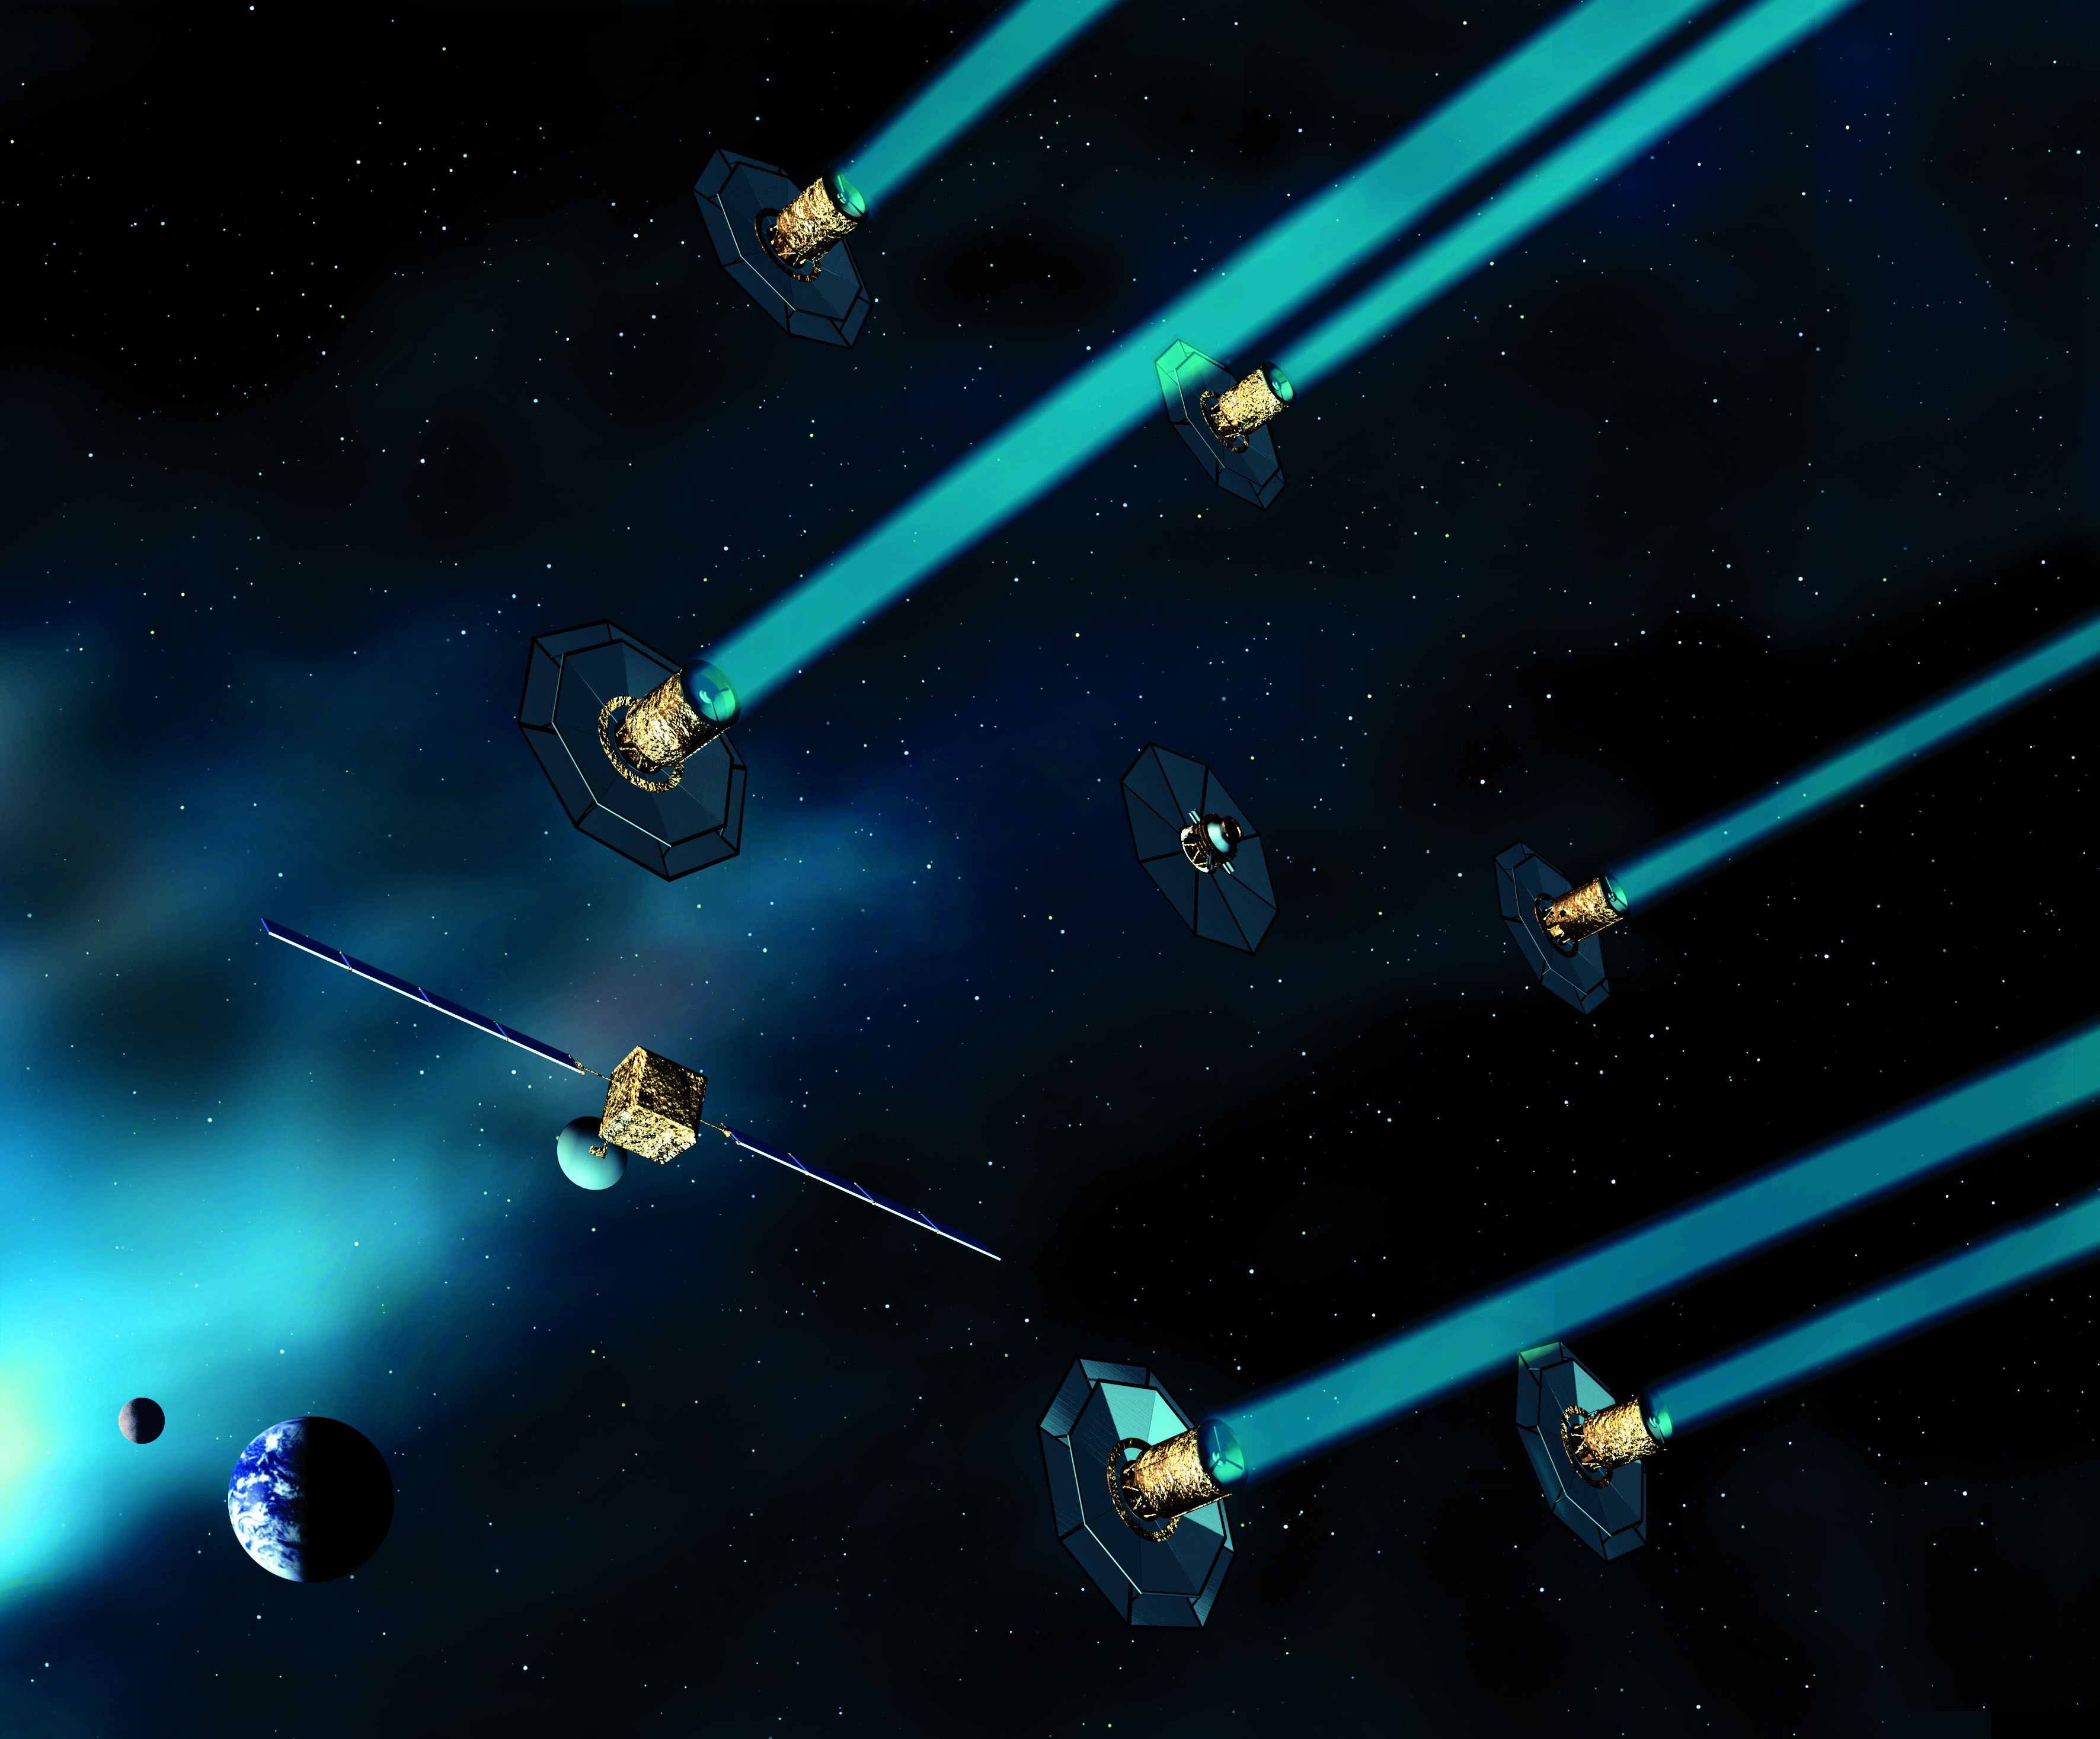
\includegraphics[width=2.4cm]{Mot_darwin1.jpg}\hspace*{0.3cm}
            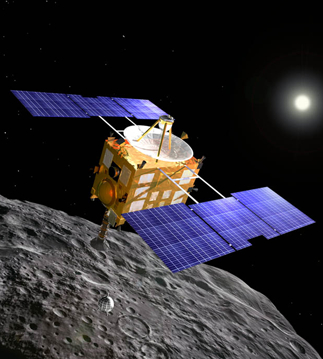
\includegraphics[width=1.81cm]{sat.jpg} \hspace*{0.3cm}
            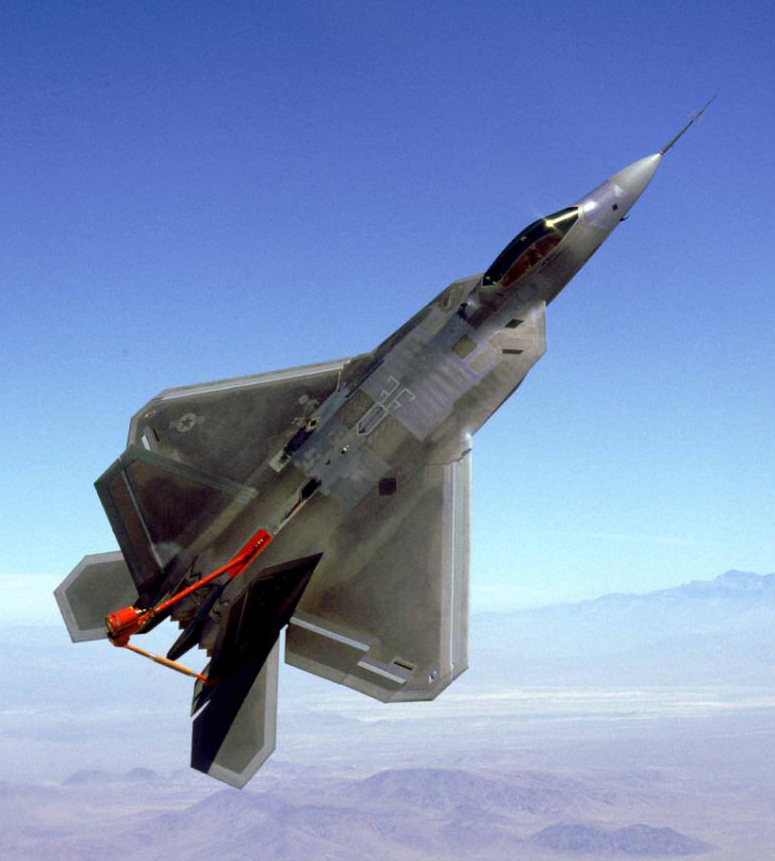
\includegraphics[width=1.8cm]{f22.jpg} \hspace*{0.3cm}
            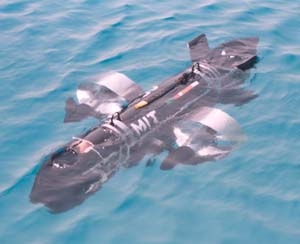
\includegraphics[width=2.49cm]{orca2b.jpg} 
            }
          	\end{figure}	
\end{frame}   %-----------------------------%



\begin{frame} %-----------------------------%
\frametitle{Geometric Control and Estimation}
\begin{itemize} 
\item Geometric Control and Estimation on Nonlinear Manifold 
	\begin{itemize} 
	\item Questions of \Emph{global nature} require global analysis for satisfactory solutions.
	\vspace*{0.1cm} 	
	\item Control and estimation systems are designed from the perspective of \Emph{differential geometry}.
%	\vspace*{0.1cm} 
%	\item ``Coordinate-invariant'' and ``intrinsic formulations''.
	\end{itemize} 
	\vspace*{0.3cm}
%\pause	
\item Geometric Control and Estimation on $\SO$	
	\begin{itemize} 
	\item \tc{purple}{No singularities} in representing large angle rotational maneuvers.
	\vspace*{0.1cm} 
	\item \tc{purple}{No ambiguities} and unwinding associated with quaternions.
	\vspace*{0.1cm} 
	\item Remarkably \tc{purple}{compact form} of equations of motion for complex aerospace systems.
	\end{itemize} 	
\end{itemize} 
\end{frame}   %-----------------------------%

\begin{frame} %-----------------------------%
\frametitle{Topological Obstruction}
\begin{itemize} 
\item Topological Obstruction of $\SO$
	\begin{itemize} 
	\item Global asymptotic stability: \\ Lyapunov stability + \Emph{global attractivity}. 	
	\vspace*{0.05cm} 
	\item \tc{purple}{No \textit{continuous} controller} can globally asymptotically stabilize an equilibrium of a attitude control system	[Bhat,~2000].
	\end{itemize} 
	\vspace*{0.2cm}	
\item Continuous Attitude Control Law
	\begin{itemize}
	\item \textit{Almost} global asymptotic stability: the region of attraction excludes only a set of zero measure. 
	\vspace*{0.05cm} 
	\item \Emph{Convergence rate is slow} when the initial state is closed to undesired equilibria.
	\end{itemize} 	
\pause	
	\vspace*{0.2cm}	
	\item Literatures
		\begin{itemize} 
		\item Attitude observer/estimator on $\SO$: [Mahony,~2008], [Vasconcelos,~2009], [Sanyal,~2012].
		\vspace*{0.05cm} 
		\item Hybrid attitude control system: [Mayhew,~2013], [Lee,~2013].
		\end{itemize}
	
\end{itemize}	
\end{frame}   %-----------------------------%


%\begin{frame} %-----------------------------%
%\frametitle{}
%\begin{itemize} \item \vspace*{0.1cm} \end{itemize} 
%\end{frame}   %-----------------------------%




\section*{Problem Formulation}
\begin{frame} %-----------------------------%
\frametitle{Problem Description}
\begin{itemize} 
\item Vector Measurements
	\begin{itemize} 
	\item Let $v_i^I\in\Sph^2$ be the unit vectors in the reference frame, for $i={1,2,\ldots,n}$ ($n\geq2$). 
	\vspace*{0.05cm}
	\item The rigid body is equipped with sensors to measure such reference directions: 
	{\small \begin{gather*} v_i^B(t)=R(t)^\T v_i^I\in\Sph^2. \end{gather*}} 
	\end{itemize}
\pause
\item Angular velocity Measurements\\
The angular velocity measurements is assumed to be corrupted with \Emph{fixed bias $\ga$}
	{\small \begin{gather*} \W_y=\W+\ga\in\Re^3. \end{gather*}} 	
\item Equation of Motion: $\dot{R}=R\hat{\W}$. 
\pause
	\begin{tcolorbox}
	Design observer to estimate the attitude $R$ of the rigid body based on these measurements with gyro bias.
	\end{tcolorbox}
\end{itemize} 
\end{frame}   %-----------------------------%

\subsection*{Problem Formulation}
\begin{frame} %-----------------------------%
\frametitle{Esitmate Frame \& Estimate Error}
\begin{itemize} 
\item Estimate Frame
	\begin{itemize} 
	\item Estimate attitude and bias are given by $\bar{R}\in\SO$, $\bar{\ga}\in\Re^3$.
	\vspace*{0.05cm}
	\item Express the reference direction $v_i^I$ with respect to the estimate frame:	
	{\small \begin{gather*} v_i^E=\bar{R}^\T v_i^I\in\Sph^2. \end{gather*}}
	\end{itemize}
%\vspace*{0.2cm}
\pause	
\item Estimate Error
	\begin{itemize} 	 	 	
	\item The discrepancy between the true attitude $R$ and the estimate attitude $\bar{R}$
	{\small \begin{gather*} \td{R}=\bar{R}^\T R\in\SO. \end{gather*}} 	
	\item Estimate Error Function 
	{\small \begin{gather*} \Psi_i=1-{v_i^E}^\T v_i^B\in\Re,\quad \Psi=\sum_{i=1}^nk_i\Psi_i\in\Re. \end{gather*}}. 
	\item Bias estimate error: $\td{\ga}=\ga-\bar{\ga}\in\Re^3$.	
	\end{itemize}  
\end{itemize} 
\end{frame}   %-----------------------------%


\begin{frame} %-----------------------------%
\frametitle{Complementary Filter [Mahony, 2008] }
%\begin{itemize} 
%\item Review [Mahony, 2008] 
	\begin{prop}[] %~~~~~Poposition~~~~~%
	{\small The complementary filter is defined as
		\begin{gather*} 
		\dot{\bar R}=\bar{R}[(\W_y-\bar{\ga})+k_R\tc{purple}{e_R}]^\vee,\quad \dot{\bar \ga}=-k_I\tc{purple}{e_R},\\
		\tc{purple}{e_R}=\sum_{i=1}^nk_i v_i^B\t v_i^E,
		\end{gather*}
	for positive constants $k_R,k_I\in\Re$.		
	}
		\begin{itemize} 
		\item There are 4 equilibria, given by
%		\vspace*{-0.1cm}
			{\footnotesize\begin{gather*} 
			(\bar R,\bar{\ga})\in\{(R,\ga),(UD_iU^\T R,\ga)\}.
			\end{gather*}}				
%		\vspace*{-0.5cm} 
		\item The desired equilibrium $(\bar R,\bar{\ga})=(R,\ga)$ is almost globally asymptotically stable.
%		\vspace*{0.05cm} 
		\item Convergence rate is slow when the initial state is close to undesired equilibria.		
		\end{itemize} 	
	\end{prop} 		
%\end{itemize} 
\end{frame}   %-----------------------------%


\begin{frame} %-----------------------------%
\frametitle{Alternative Form of Error Function}
\begin{itemize} 
\item Estimate Error Function
	{\footnotesize 
	\begin{gather*}  \Psi=\sum_{i=1}^nk_i(1-{v_i^E}^\T v_i^B)=\sum_{i=1}^nk_i-\tr[\bar{R}^\T\Emph{K}R],\\
	K=\sum_{i=1}^nk_iv_i^I{v_i^I}^\T=K^\T =\Emph{\sum_{i=1}^3\lam_is_is_i^\T}.
	\end{gather*}} 	
As $K$ is symmetric and positive-(semi)definite, we have
	{\footnotesize 
	\begin{gather*}  
	K=UGU^\T=\left[\begin{array}{ccc}|&|&|\\s_1& s_2& s_3\\|&|&| \end{array}\right] \left[\begin{array}{ccc}\lam_1&0&0\\0&\lam_2&0\\0&0&\lam_3\end{array}\right] \left[\begin{array}{ccc}-&s_1&-\\-& s_2& -\\-& s_3&- \end{array}\right],
	\end{gather*}}
%	\vspace*{-0.3cm} 
	where $U\in\SO$ and $G$ is defined by eigenvalues.
\pause
\item Using $\tc{purple}{b_i}=R^\T s_i$ and $\tc{purple}{\bar{b}_i}=\bar{R}^\T s_i$,
%	{\small\begin{gather*} 
%	b_i=R^\T s_i,\quad \bar{b}_i=\bar{R}^\T s_i.	
%	\end{gather*}} 	
the estimate function can be rewritten as 
	{\small\begin{gather*} 
	\Psi=\sum_{i=1}^3 \lam_i(1-\bar{b}_i^\T b_i).
	\end{gather*}}
\end{itemize} 
\end{frame}   %-----------------------------%

\begin{frame} %-----------------------------%
\frametitle{Motivation of Hybrid Observer}
\begin{itemize}
\item Necessity of Hybrid System
\begin{itemize} 
\item Equilibria configuration
	\begin{itemize} 
	\item 1 desired equilibrium: $(\bar{b}_1,\bar{b}_2,\bar{b}_3)=(b_1,b_2,b_3)$
	\item 3 undesired equilibria:
	{\small\begin{gather*} 
	(\bar{b}_1,\bar{b}_2,\bar{b}_3)=(b_1,-b_2,-b_3),\qquad\qquad\\
	(\bar{b}_1,\bar{b}_2,\bar{b}_3)=(-b_1,b_2,-b_3),\qquad\qquad\\
	(\bar{b}_1,\bar{b}_2,\bar{b}_3)=(-b_1,-b_2,b_3).\qquad\qquad
	\end{gather*}}
	\end{itemize} 
\vspace*{0.1cm} 
\pause
\item Error functions for hybrid observer
	\begin{itemize} 
	\item Nominal Mode: same as [Mahony, 2008].
	\vspace*{0.05cm} 
	\item \Emph{Expelling Mode}: 2 expelling modes are designed to steer the attitude configuration away from 3 undesired equilibria.	 
	\end{itemize}
\vspace*{0.2cm} 	
\item Topological obstruction is avoided due to discontinuity.	
%\vspace*{0.1cm} 
%\item Starting from nominal mode, switching logic is triggered when the estimate attitude is near to undesired equilibria.	
\end{itemize} 
\end{itemize} 
\end{frame}   %-----------------------------%

\begin{frame} %-----------------------------%
\frametitle{Hybrid Observer -- Switching Logic}
\only<1>{
\begin{minipage}[t]{0.50\linewidth}
	\begin{itemize} 
	\vspace*{-0.1cm}
	\item Nominal Mode
 	\begin{figure} %figure%
 	\hspace*{-1.5cm}   
    \includegraphics[width=1.1\columnwidth]{4_Nominal.pdf}
  	\hspace*{1.5cm}   
  	\end{figure}	
  	\vspace*{0.05cm}
	\end{itemize}	
\end{minipage}\hfill
%\begin{minipage}[t]{0.50\linewidth}
%	\begin{itemize} 
%	\item Expelling Mode
%	\begin{figure} %figure%
%	\hspace*{-0.8cm}
%    \centering\includegraphics[width=1.1\columnwidth]{4_Expell.pdf}
%    \hspace*{0.8cm}
%  	\end{figure}	
%	\end{itemize}
%\end{minipage}
}
\only<2>{
\begin{minipage}[t]{0.50\linewidth}
	\begin{itemize} 
	\item Nominal Mode
%	\vspace*{-0.1cm}
 	\begin{figure} %figure%
 	\hspace*{-1.5cm}   
    \includegraphics[width=1.1\columnwidth]{4_Nominal.pdf}
  	\hspace*{1.5cm}   
%  	\vspace*{0.4cm}
  	\end{figure}
	\end{itemize}	
\end{minipage}\hfill
\begin{minipage}[t]{0.50\linewidth}
	\begin{itemize} 
	\item Expelling Mode
	\begin{figure} %figure%
	\hspace*{-0.8cm}
    \centering\includegraphics[width=1.1\columnwidth]{4_Expell.pdf}
    \hspace*{0.8cm}
    \vspace*{0.4cm}
  	\end{figure}	
	\end{itemize}
\end{minipage}
}
\end{frame}   %-----------------------------%

%\begin{frame} %-----------------------------%
%\frametitle{Hybrid Observer}
%\begin{itemize} 
%\item Once the estimate attitude is away from undesired equilibria, error function is switched back to nominal mode.
%\pause
%\vspace*{0.1cm} 
%\item Topological obstruction is avoided due to discontinuity. 
%\vspace*{0.1cm} 
%\item Hysteresis-based switching for robustness of the system. 
%
%\end{itemize} 
%\end{frame}   %-----------------------------%


\section*{Attitude Observer with Global Asymptotic Stability}
\begin{frame} %-----------------------------%
\frametitle{Hybrid Observer Design}
\begin{prop}[] %~~~~~Poposition~~~~~%
{\small The hybrid attitude observer is defined as
\vspace*{-0.15cm}
	\begin{gather*} 
	\dot{\bar R}=\bar{R}[(\W_y-\bar{\ga})+k_R\tc{purple}{e_H}]^\vee,\quad \dot{\bar \ga}=-k_I\tc{purple}{e_H},\quad e_H=\sum_{i=1}^n\lambda_i e_{H_i},
	\end{gather*}
\vspace*{-0.15cm}
where the $i$-th hybrid innovation term $e_{H_i}$ is given by	
	\begin{align*}
  	e_{H_1}&=\begin{cases}
               b_1\t\bar{b}_1 & \text{if}\quad \m=\Ra,\Rb,\\
               -\be(b_3\t\bar{b}_1) & \text{if}\quad \m=\Rc,\\
            \end{cases} 
  	\\
  	e_{H_2}&=\begin{cases}
               b_2\t\bar{b}_2 & \text{if}\quad \m=\Ra,\Rc,\\
               -\be(b_3\t\bar{b}_2) & \text{if}\quad \m=\Rb,\\
            \end{cases}
  	\\          
  	e_{H_3}&= b_3\t\bar{b}_3  \qquad\quad\text{for}\quad \m=\Ra,\Rb,\Rc. 
	\end{align*}
Then, the desired equilibrium $(\bar{R},\bar{\ga})=(R,\ga)$ is globally asymptotically stable, and the number of discrete jumps is finite.
}
\end{prop} 
%\begin{itemize} 
%\item 
%\end{itemize} 
\end{frame}   %-----------------------------%

\begin{frame} %-----------------------------%
\frametitle{Hysteresis Switching}
\begin{itemize} 
\item Switching Logic
	\begin{itemize} 
	\item The observer is switched into the new mode that yields the minimum error function
		{\small\begin{gather*}
		\rho(\bar R)=\min_{\m\in\M}\{\Psi_\m(\bar R)\},\quad \text{for } \M\in\{\Ra,\Rb,\Rc\}.
		\end{gather*}}	
	\item $\Psi_m:$ current error function; $\rho:$ minimum error function.		
	\vspace*{0.1cm}	
	\item It may cause \Emph{chattering} due to measurement noise if the switch events happen whenever $\Psi_\m>\rho$. 			
	\end{itemize}
\pause	
\vspace*{0.2cm}
\item Hysteresis Gap
	\begin{itemize}
	\item A positive hysteresis gap: $\delta\in\Re$. 
	\vspace*{0.1cm}
	\item Switching is triggered if  \tc{purple}{$\Psi_\m-\rho\geq\delta$}. 
	\vspace*{0.1cm}
	\item Increase the \Emph{robustness} of the observer.
	\end{itemize} 
\end{itemize} 		
\end{frame}   %-----------------------------%




\section*{Numerical Analysis}
\begin{frame} %-----------------------------%
\frametitle{Numerical Integraton}
\begin{itemize} 
\item Numerical Integration Error
	\begin{itemize} 
	\item $\SO$ has \Emph{higher cumulative error} during numerical integration since to the group operation is not additive. Let $R_1,R_2\in\SO$,
		{\small\begin{gather*}
		R_1+R_2\notin\SO,\qquad R_1R_2\in\SO.
		\end{gather*}}	
	\item Conventional Runge-Kutta
		{\small\begin{gather*}
		\bar{R}_{n+1}'=\bar{R}_{n}+hK.
		\end{gather*}}				
	\end{itemize}
\pause	
\item Solutions
	\begin{itemize}
	\item Reduce error tolerance numerically: \\
	\begin{alltt}
	{\scriptsize OdeOption=odeset('RelTol',1e-10,'AbsTol',1e-10)}.
	\end{alltt}
	\item \Emph{Geometric numerical integrator}: preserve the structure of $\SO$ during simulation.
	\end{itemize} 
\end{itemize} 		
\end{frame}   %-----------------------------%


\begin{frame} %-----------------------------%
\frametitle{Geometric Numerical Integrator}
\only<1>{
	\begin{itemize} 
	\item Geometric Runge-Kutta (2nd order)
	\begin{itemize}
	\item Intermediate update:\\
	{\small $\bar{R}_{n+1}'=\exp^{hK_{{\bar R}_1}}\bar{R}_{n}$,~ $K_{{\bar R}_1} =(\bar{R}_{n}\bar{\Omega}_n)^\wedge$.}\\
	{\small $\bar\ga_{n+1}'=\bar\gamma_n+hK_{{\bar\gamma}_1}$,~ $K_{{\bar\gamma}_1}=-k_Ie_{H_n}(R_n,\bar{R}_n)$.}\\
%		{\small\begin{gather*} 
%		\bar{R}_{n+1}'=\exp^{hK_{{\bar R}_1}}\bar{R}_{n},\qquad K_{{\bar R}_1} =(\bar{R}_{n}\bar{\Omega}_n)^\wedge\qquad\\ 
%		\bar\ga_{n+1}'=\bar\gamma_n+hK_{{\bar\gamma}_1},\qquad K_{{\bar\gamma}_1}=-k_Ie_{H_n}(R_n,\bar{R}_n)
%		\end{gather*}}
\vspace*{0.2cm}		
	\item Full-step update:	
	{\small\begin{gather*} 
	\bar{R}_{n+1}=\exp^{\frac{1}{2}h(K_{{\bar R}_1}+K_{{\bar R}_2})}\bar{R}_{n},\quad   \bar{\ga}_{n+1}=\bar\ga_n+\frac{1}{2}h(K_{\bar{\ga}_1}+K_{\bar{\ga}_2}).
	\end{gather*}}
	\end{itemize}				
	\end{itemize}
\vspace*{4.2cm}			
}
\only<2>{	
	\begin{itemize} 
	\item Geometric Runge-Kutta (2nd order)
	\begin{itemize}
	\item Intermediate update:\\
	{\small $\bar{R}_{n+1}'=\exp^{hK_{{\bar R}_1}}\bar{R}_{n}$,~ $K_{{\bar R}_1} =(\bar{R}_{n}\bar{\Omega}_n)^\wedge$.}\\
	{\small $\bar\ga_{n+1}'=\bar\gamma_n+hK_{{\bar\gamma}_1}$,~ $K_{{\bar\gamma}_1}=-k_Ie_{H_n}(R_n,\bar{R}_n)$.}\\
\vspace*{0.2cm}		
	\item Full-step update:	
	{\small\begin{gather*} 
	\bar{R}_{n+1}=\exp^{\frac{1}{2}h(K_{{\bar R}_1}+K_{{\bar R}_2})}\bar{R}_{n},\quad   \bar{\ga}_{n+1}=\bar\ga_n+\frac{1}{2}h(K_{\bar{\ga}_1}+K_{\bar{\ga}_2}).
	\end{gather*}}
\vspace*{-0.4cm}	 
	\begin{figure} %figure%
	\hspace*{-0.8cm}
    \centering\includegraphics[width=0.45\columnwidth]{fig_4_ni150.pdf}
    \hspace*{0.8cm}
  	\end{figure}	
\vspace*{-0.3cm}  		
  	\item Result: eliminate cumulative error without reducing tolerance error.	
	\end{itemize}				
	\end{itemize}
}		
\end{frame}   %-----------------------------%





\begin{frame} %-----------------------------%
\frametitle{Numerical Examples}
	\begin{itemize} 
	\item Without Gyro Bias
		\begin{figure}
		\centering	
		\hspace*{-0.1\columnwidth}
		\subfigure{\includegraphics[width=0.29\columnwidth]{fig_4_att.pdf}}
%		\hspace*{-0.03\columnwidth}
		\subfigure{\includegraphics[width=0.29\columnwidth]{fig_4_sw.pdf}}
%		\hspace*{-0.03\columnwidth}			
		\subfigure{\includegraphics[width=0.29\columnwidth]{fig_4_eR.pdf}}								
		\end{figure}	
	\item With Gyro Bias
		\begin{figure}
		\centering	
		\hspace*{-0.11\columnwidth}
		\subfigure{\includegraphics[width=0.27\columnwidth]{fig_4bia_att.pdf}}
		\hspace*{-0.048\columnwidth}
		\subfigure{\includegraphics[width=0.27\columnwidth]{fig_4bia_sw.pdf}}
		\hspace*{-0.048\columnwidth}			
		\subfigure{\includegraphics[width=0.27\columnwidth]{fig_4bia_eR.pdf}}	
		\hspace*{-0.048\columnwidth}			
		\subfigure{\includegraphics[width=0.27\columnwidth]{fig_4bia_bE.pdf}}						
		\end{figure}		
	\end{itemize}	
\end{frame}   %-----------------------------%

\begin{frame} %-----------------------------%
\frametitle{Experimental Validation} 
	\begin{itemize} 
	\item Fully-Actuated Hexdrotor
	\end{itemize}
		\begin{figure}
		\centering	
%		\hspace*{-0.05\columnwidth}
		\subfigure{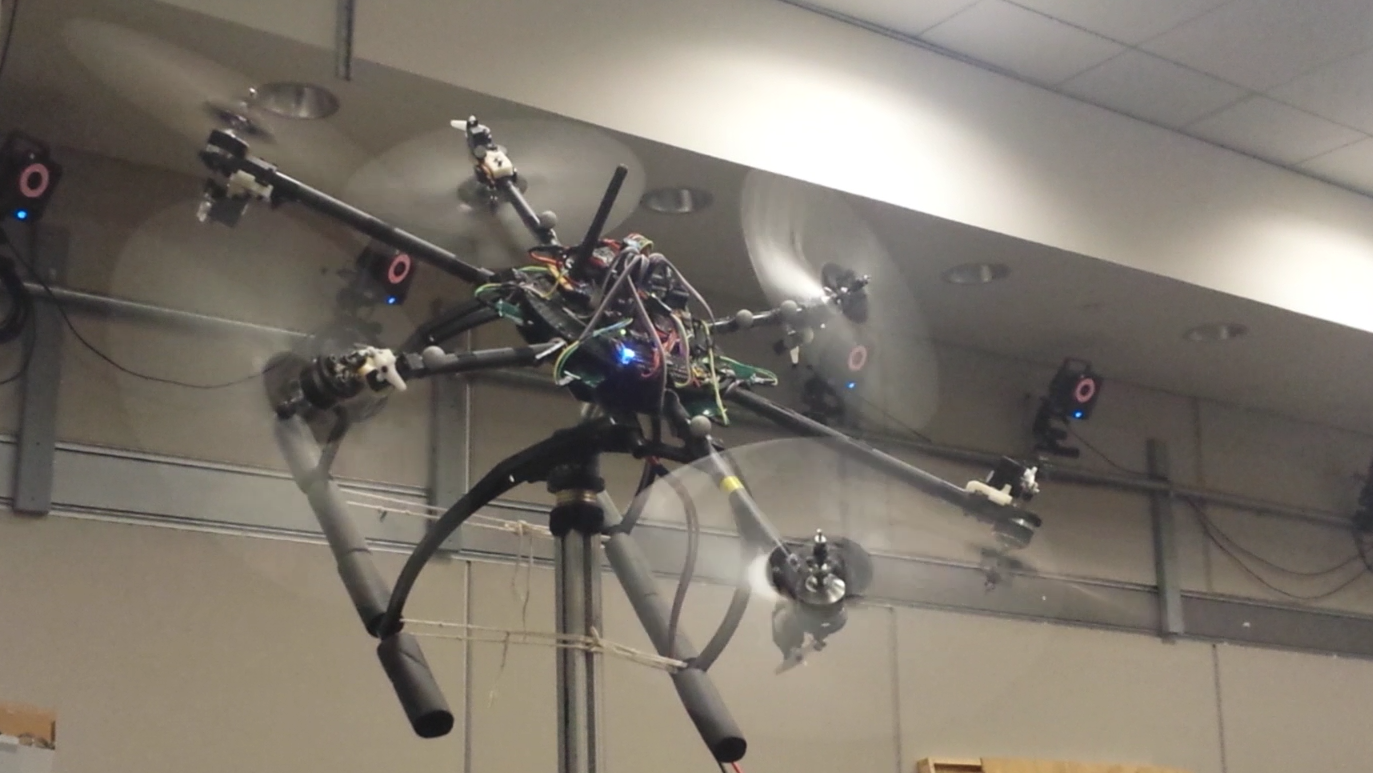
\includegraphics[height=0.22\columnwidth]{fig_4_hex1.pdf}}
		\hspace*{0.05\columnwidth}
		\subfigure{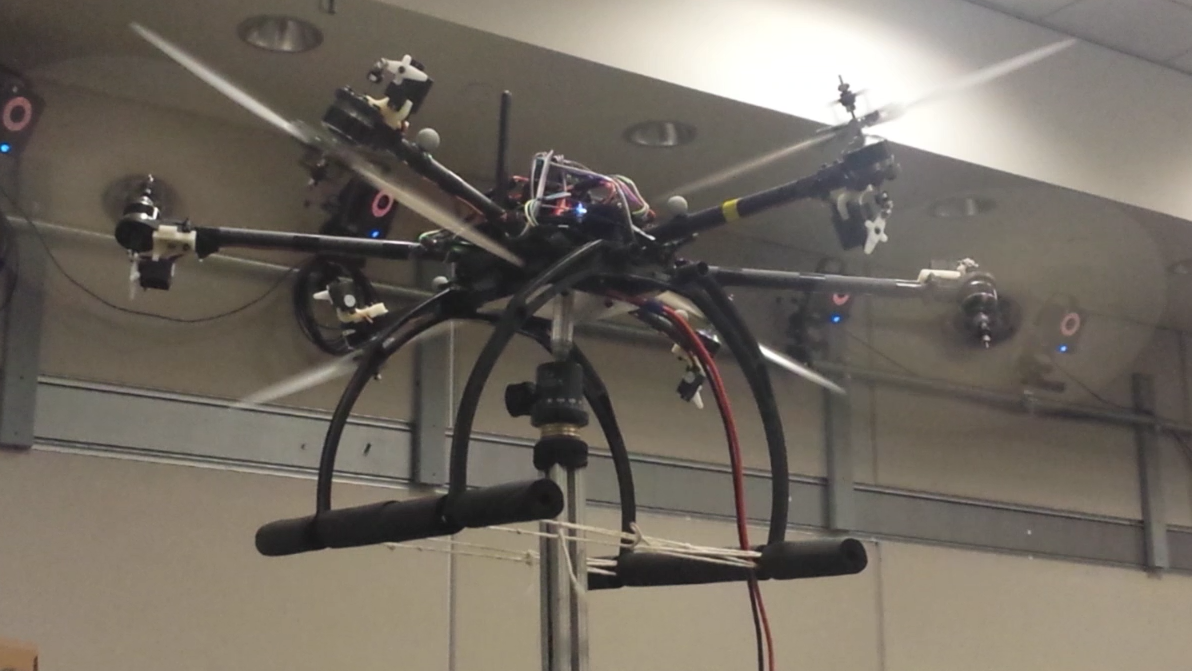
\includegraphics[height=0.22\columnwidth]{fig_4_hex2.pdf}}					
		\end{figure}
	\begin{figure} %figure%
%	\hspace*{-0.8cm}
    \centering\includegraphics[width=0.45\columnwidth]{fig_4_hex3.pdf}
%    \hspace*{0.8cm}
  	\end{figure}		
\end{frame}   %-----------------------------%


\begin{frame} %-----------------------------%
\frametitle{Experimental Result} 
\centerline{
\includemovie[poster]{80mm}{60mm}{Defense.mov}
}
\end{frame}   %-----------------------------%

%\subsection*{}
\begin{frame} %-----------------------------%
\frametitle{Conclusions \& Contributions}
\begin{itemize} 
\item Conclusions
	\begin{itemize} 
	\item Substantially faster convergence rate.
	\vspace*{0.15cm}
	\item Initial guess does NOT have to be close to the true value of the state. 	
	\vspace*{0.15cm} 
	\item Corrupted angular velocity is compensated.
	\vspace*{0.15cm}
	\item The estimated attitude evolves on the special group.
	\end{itemize} 
\vspace*{0.3cm}
\pause
\item Contribution
	\begin{itemize} 
	\item First attitude observer with global asymptotic stability.
	\vspace*{0.15cm} 
	\item Hybrid attitude observer with straightforward and intuitive switching logic.
%	\vspace*{0.1cm}
%	\item  
%	\vspace*{0.1cm} 	 
	\end{itemize}  
\end{itemize} 
\vspace*{0.6cm}
\end{frame}   %-----------------------------%


%\begin{frame} %-----------------------------%
%\frametitle{}
%\begin{itemize} \item \vspace*{0.1cm} \end{itemize} 
%\end{frame}   %-----------------------------%
%\begin{tcolorbox}\end{tcolorbox}






%\begin{frame} %-----------------------------%
%\frametitle{}
%  \begin{itemize} \item \vspace*{0.1cm} \end{itemize} 
%\end{frame}   %-----------------------------%
%=======================================================%
\end{document}
